%%%%%%%%%%%%%%%%%%%%%%%%%%%%%%%%%%%%%%%%%%%%%%%%%%%%%%%%%%%%%%%%%%%%%%%%%%%%%%%%%%%%%%%%%%%%%%%%%%%%%%%%%%%%
\section{Applications} \label{sec:apps}
Our on-demand sketch-based segmentation algorithm is a general technique that can drive various modeling applications. Here we describe some potential applications. Some of these applications directly use 2D contour queries (sketches). Other applications use our algorithm as an efficient partial matching method, where a 3D query is represented by an informative 2D contour.

\paragraph*{Sketch-driven assembly-based modeling.} A direct application of our technique is sketch based part composition~\cite{sketchbasedcompositionfunkhousersbim2008}. As our method does not rely on a pre-segmented database, it can retrieve more diverse parts for composition. Our method can also improve the expressiveness of such a system, as the user can draw complex sketches while still retrieving correctly matching parts. As shown in Figure \ref{fig:CTModels}, our method can create detailed creative shapes.

\begin{figure}\centering
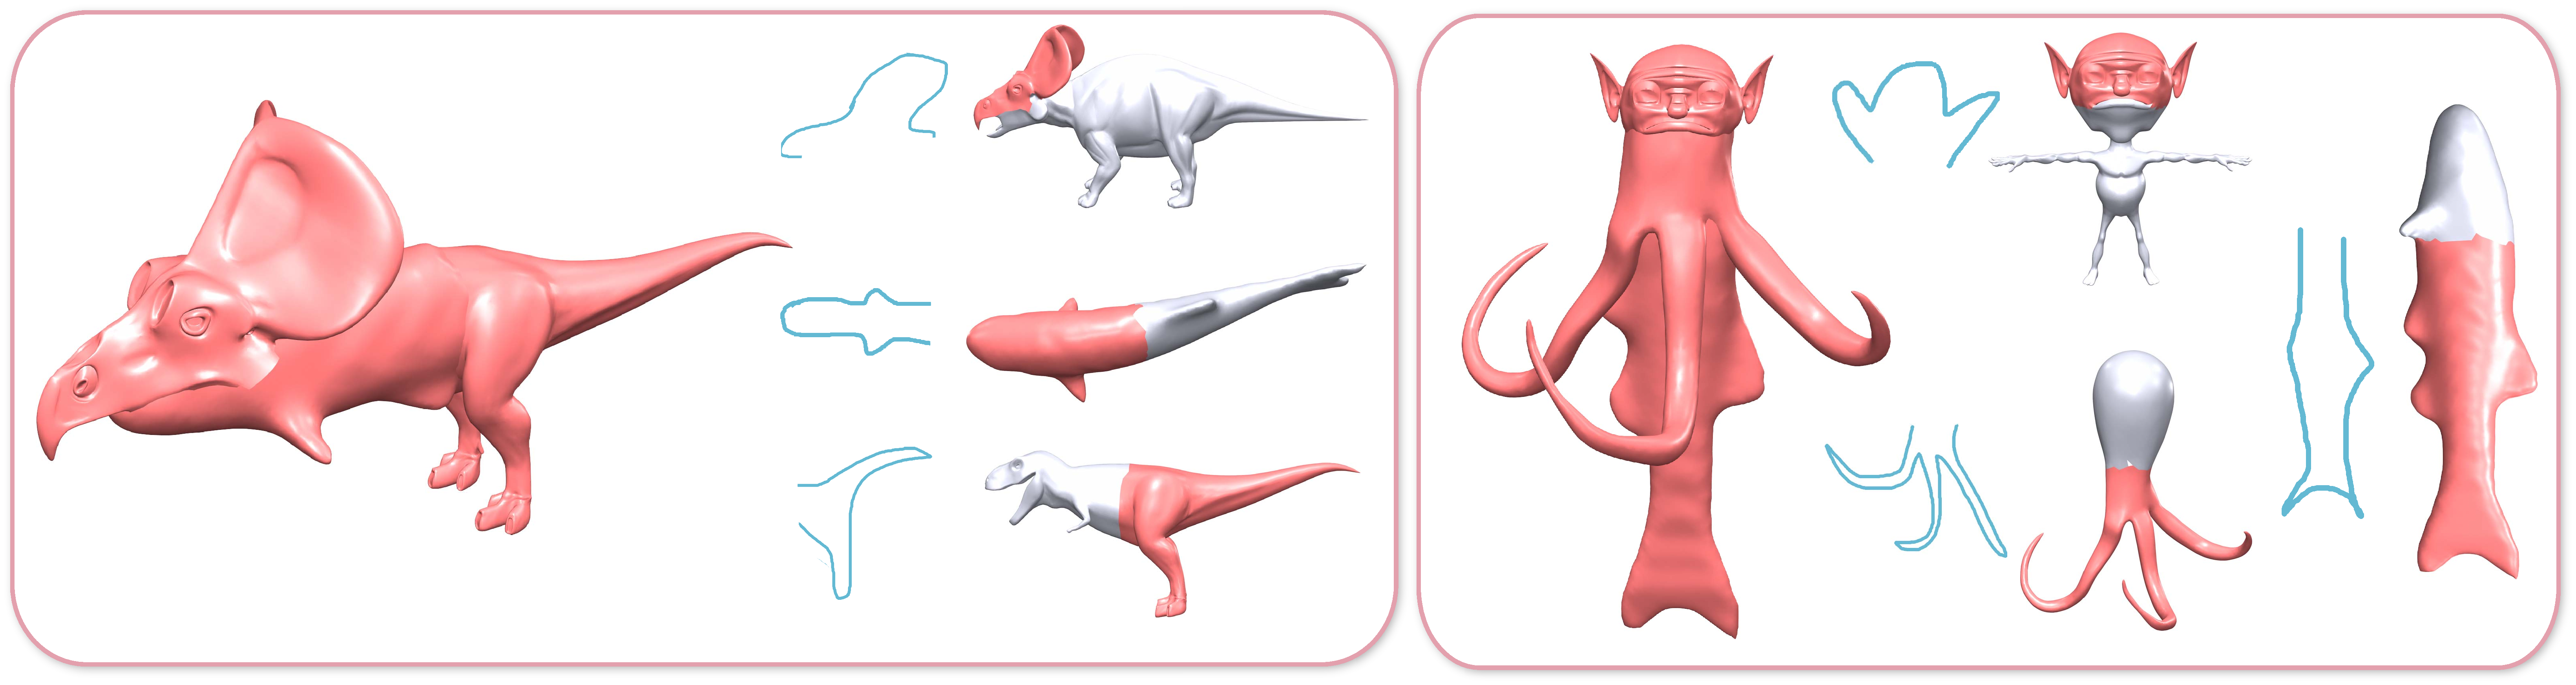
\includegraphics[width=1.05\linewidth]{./Material/CTModels.pdf}
\caption{Examples of sketch-driven assembly-based modeling. In each subfigure, we show the designed models (red), the user's sketches (blue), and the part suggestions selected by the user.}\label{fig:CTModels}
\end{figure}

\begin{figure}\centering
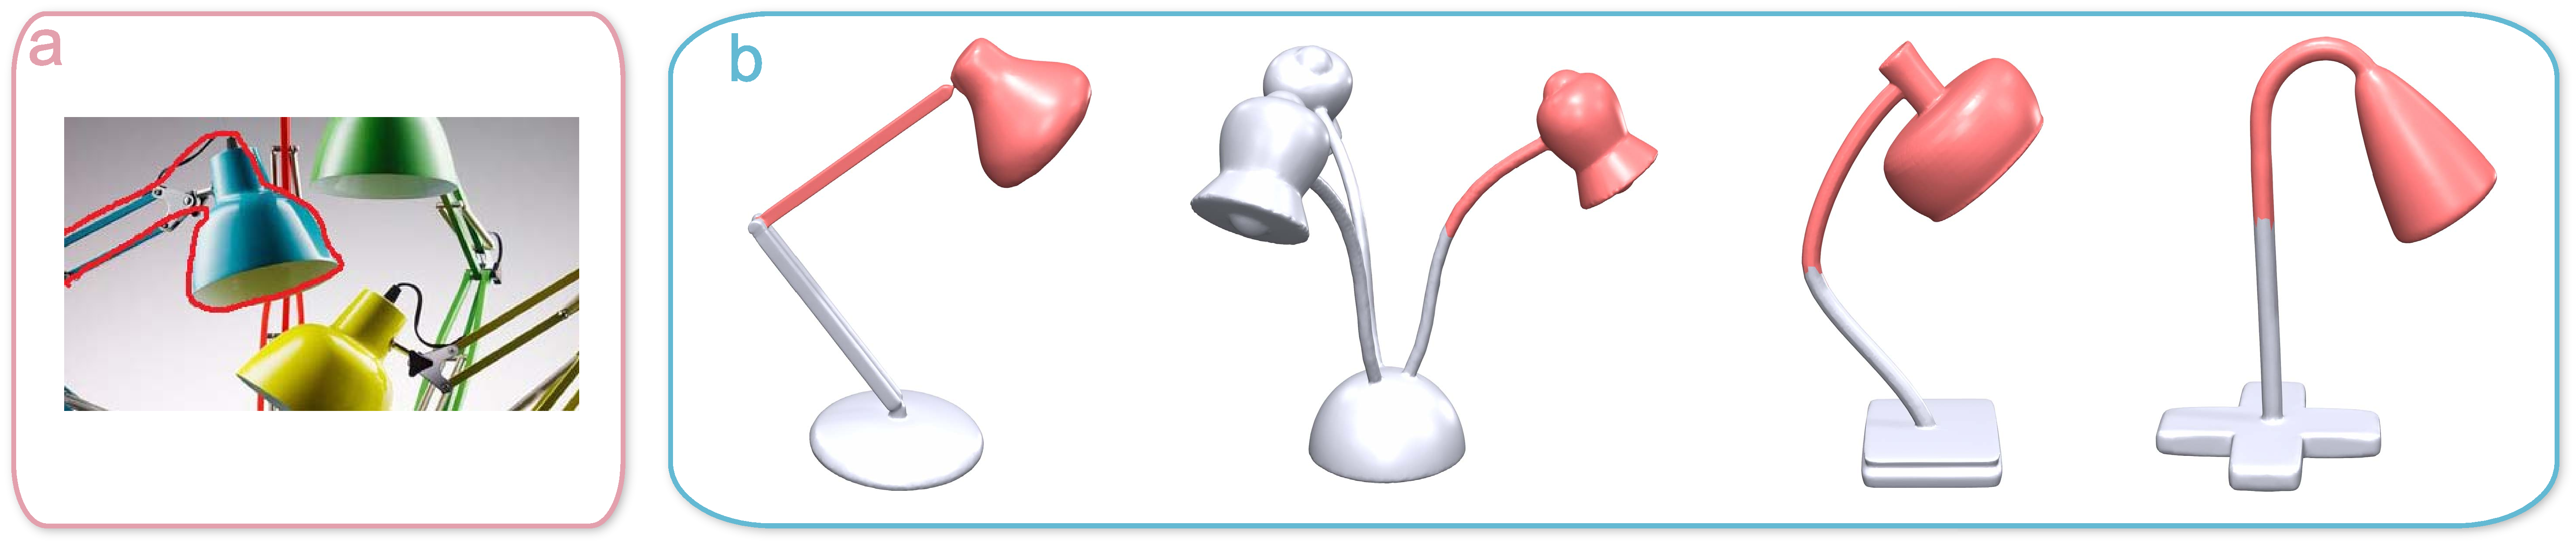
\includegraphics[width=1.05\linewidth]{./Material/Sketch2Scene.pdf}
\caption{Example of contour-driven shape completion. Given a photograph of an occluded lamp, the user traces the outer boundary of the visible portion. This trace is used as the query contour. Our algorithm retrieves possible completions for the object from a database of lamps. (Photo: Xavier Young)}\label{fig:Sketch2Scene}
\end{figure}

\paragraph*{Contour-driven shape completion.} Our algorithm can be used to suggest possible completions for occluded objects in images, an important application in computer vision and image editing. Given a photograph with an occluded object, we manually or automatically trace the boundary of the visible portion and use this trace as input to our algorithm, which retrieves possible completions of the shape from the database. Here, 2D-3D partial matching directly helps us infer the occluded portion. The process is illustrated in Figure \ref{fig:Sketch2Scene}. Alternatively, instead of starting with a photo, the user may directly draw a novel sketch with some occluded components, for example when constructing a complex 3D scene by sketching~\cite{KunXu2013}. Here, too, our algorithm can be used to help recover hidden geometry.

\begin{figure}\centering
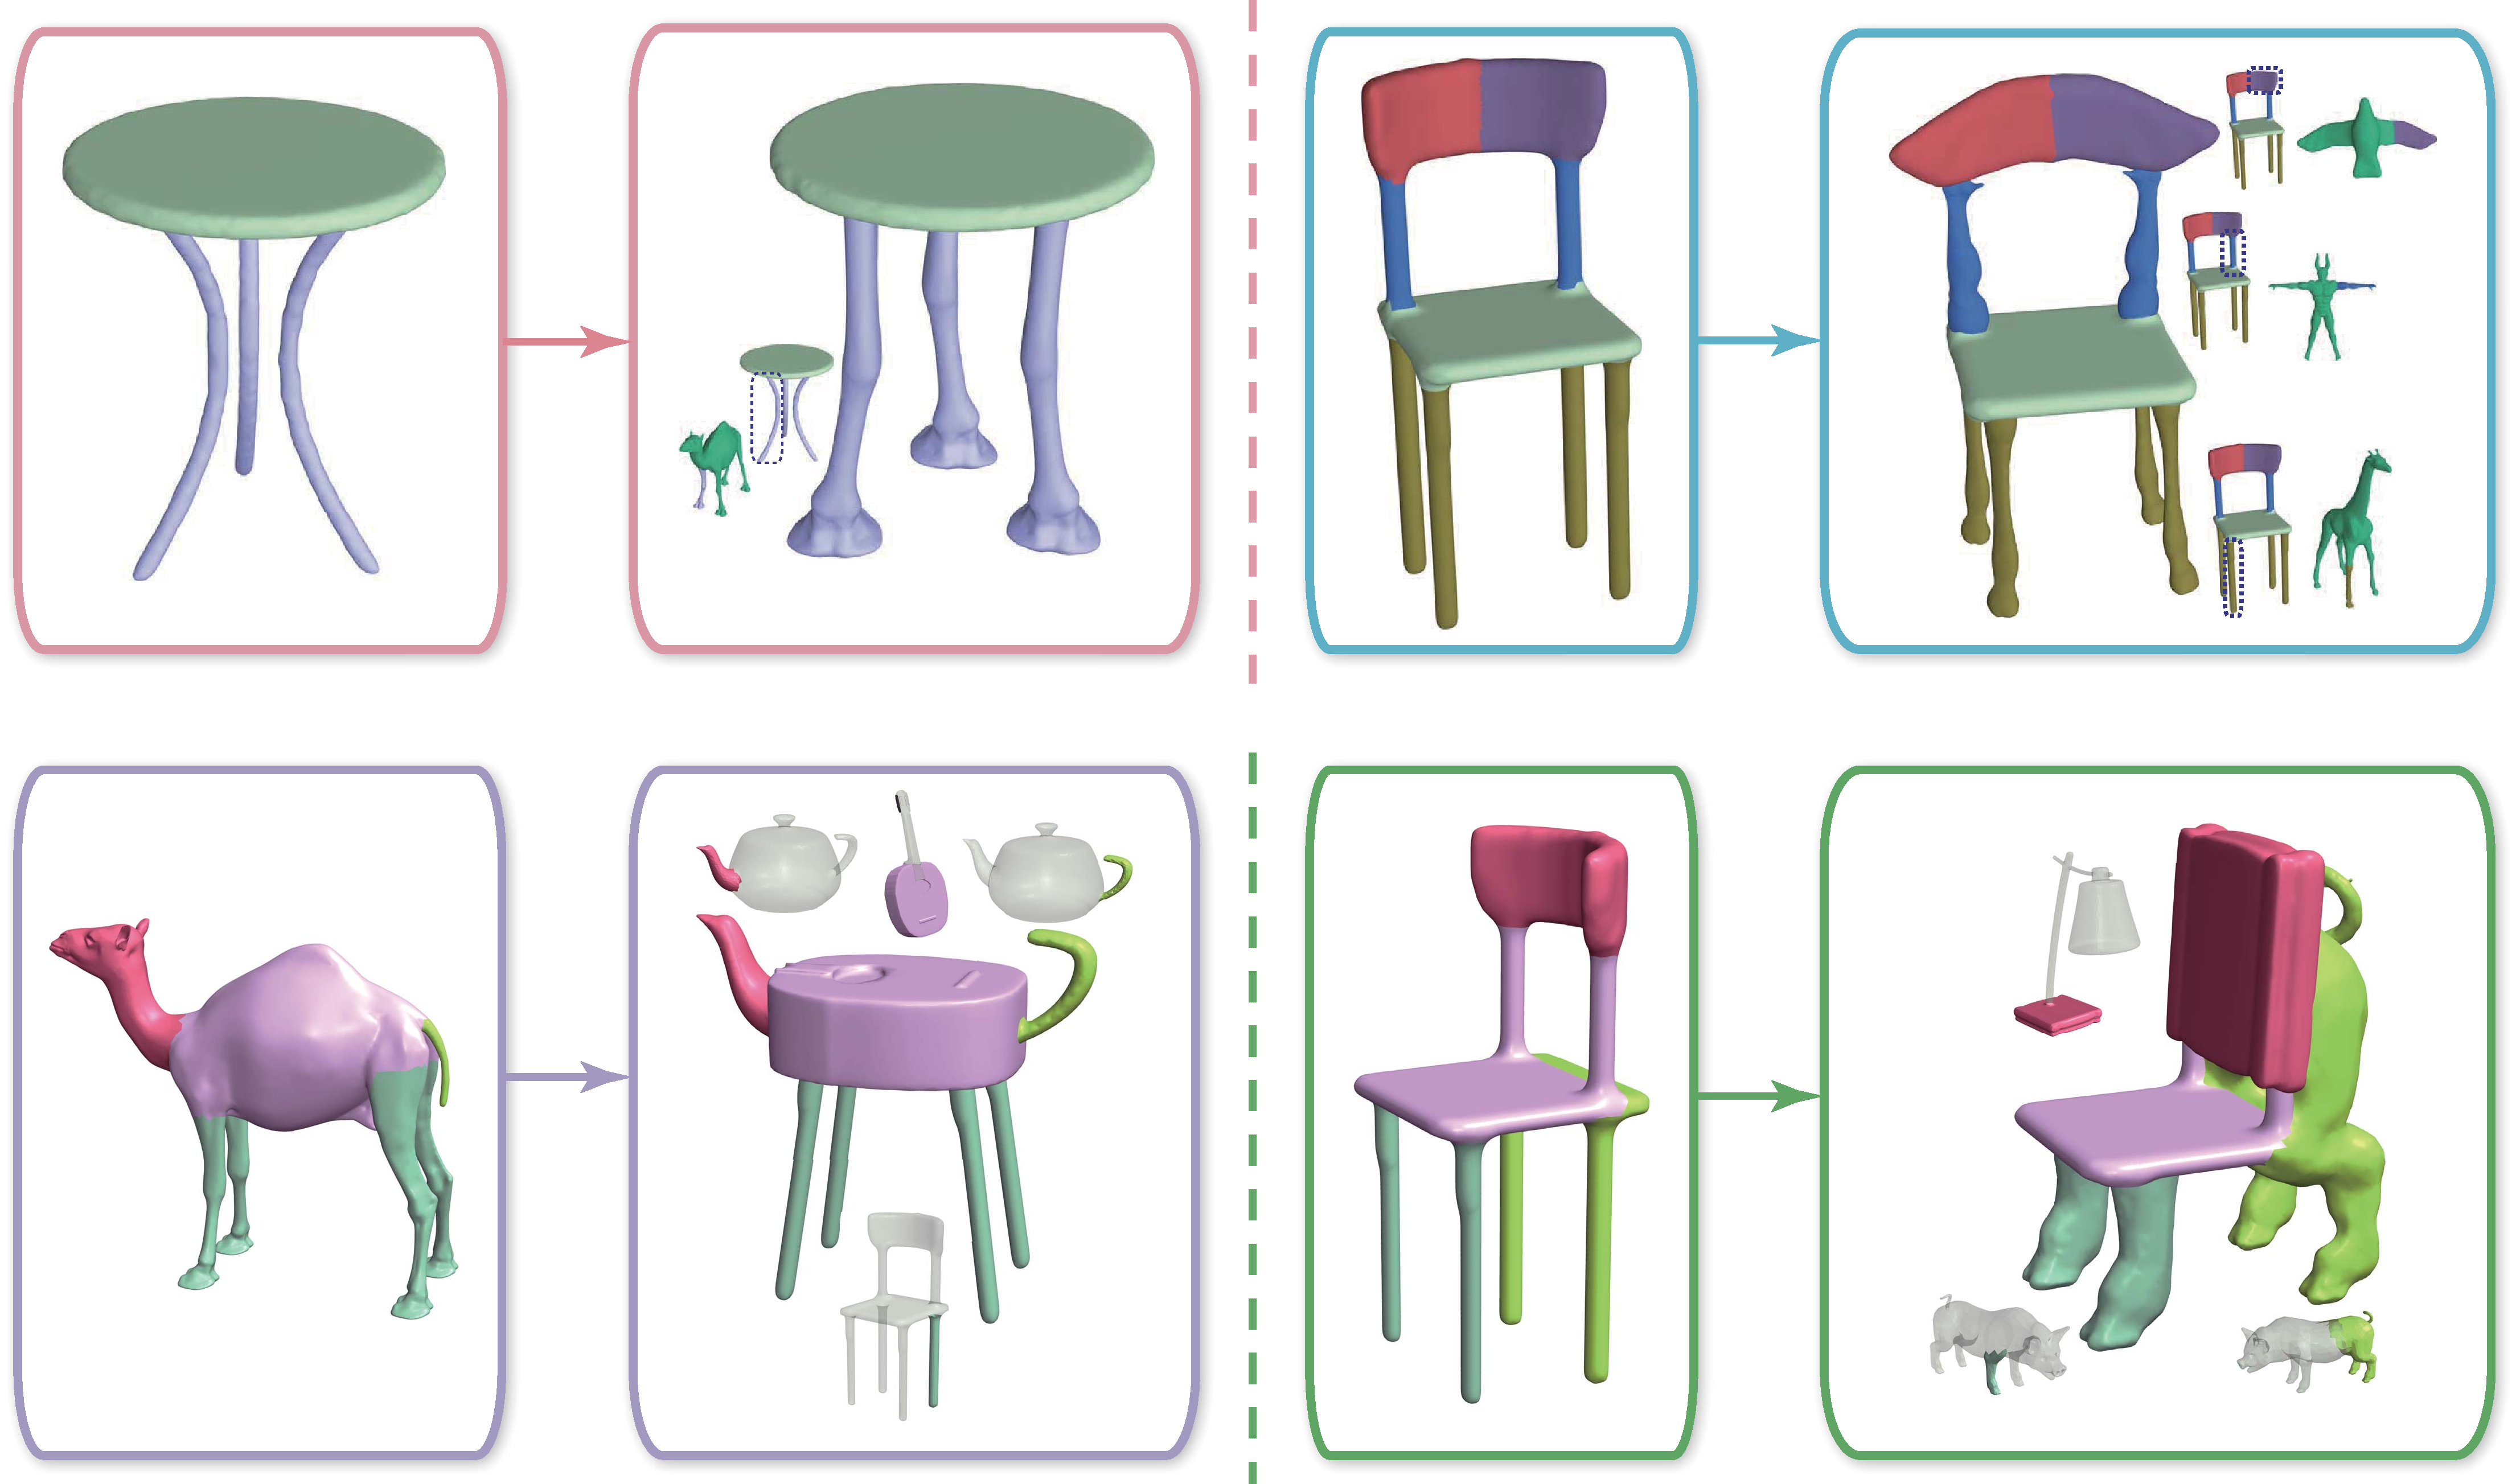
\includegraphics[width=\linewidth]{./Material/ShapeVariation.pdf}
\caption{Examples of shape variations created with our method. Given a segmented model (left), we can use one part as the query to retrieve similar parts from the database. The selected retrieved part is composited with the non-query parts to create a new shape (right) with the same layout as the original shape.}\label{fig:SegedAsInput}
\end{figure}

\paragraph*{Photo-driven part-based modeling.} \hl{Our algorithm can be used to ressemble the 3D shape in the photo. Given the photo, the use draw sketch, tracing the contour of the part, our method retrieves candidate parts from the database. The user select the appropriate parts and ressemble the 3D shape in the photo. Figure } \ref{fig:PhotoModeling}\hl{ shows an example.}

\begin{figure}\centering
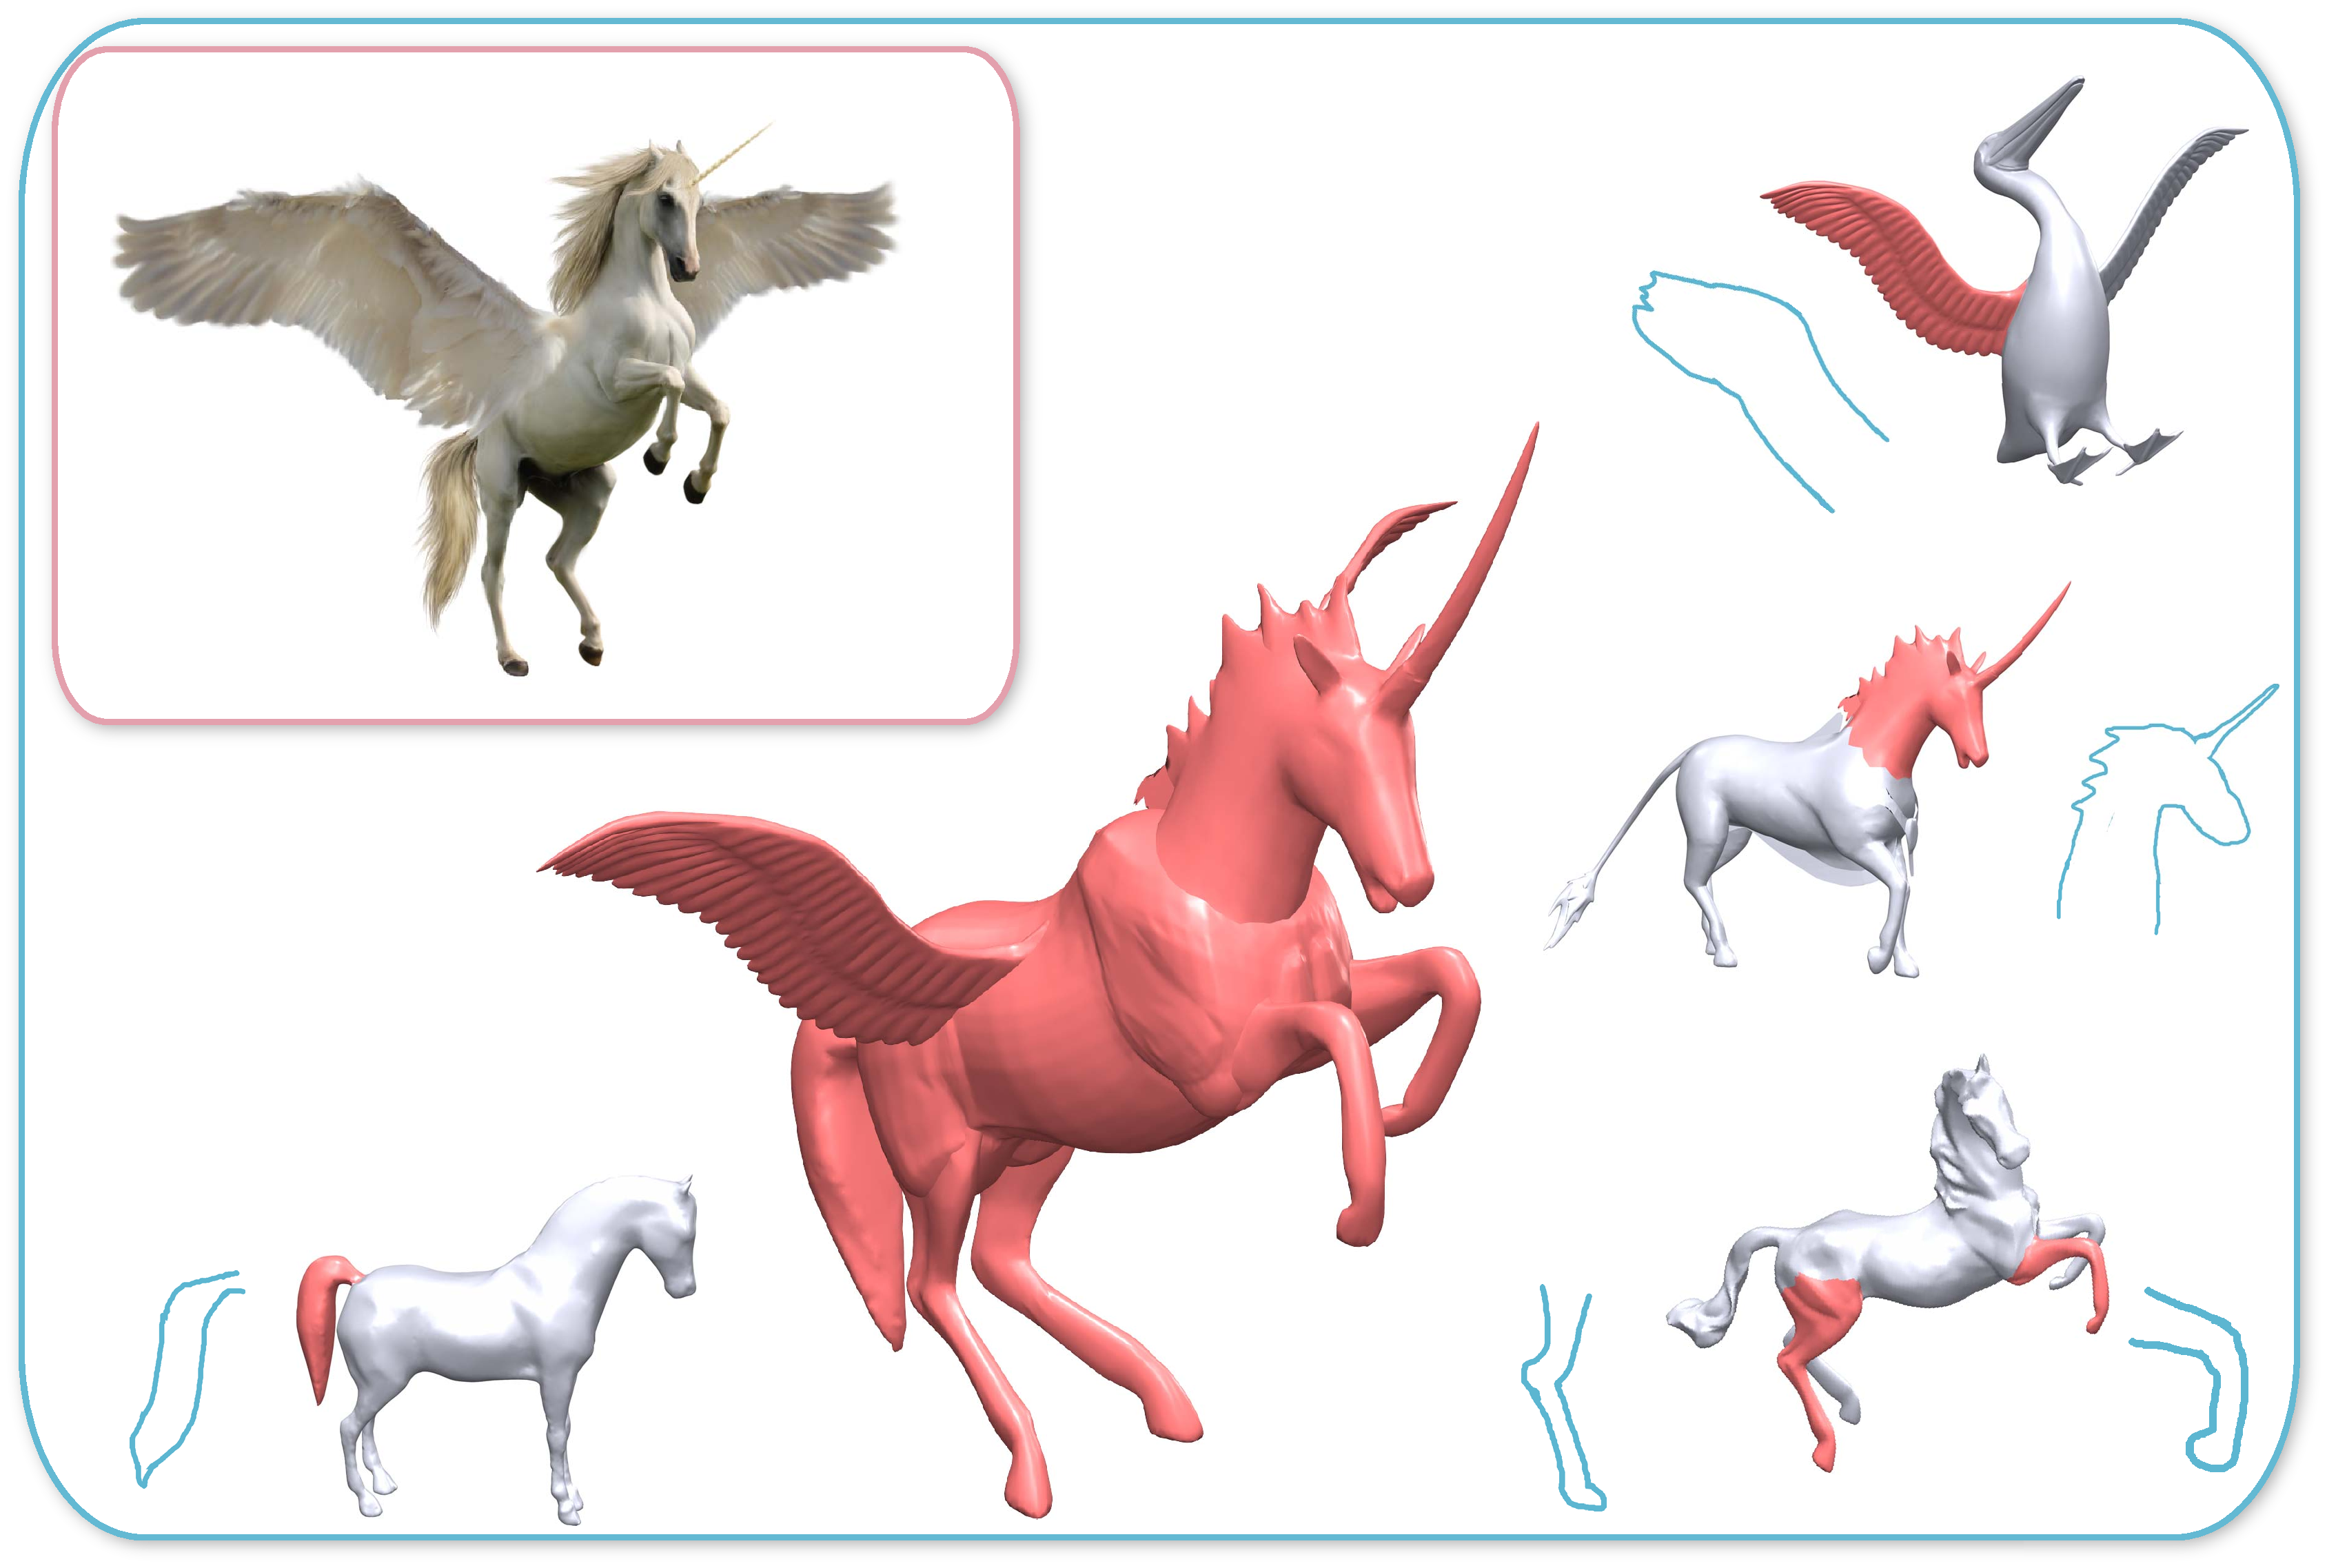
\includegraphics[width=\linewidth]{./Material/PhotoDrivenModeling.pdf}
\caption{Example of photo-driven part-based modeling. Given the photo (on the top left corner), the user sketches the contour of each part of the shape. Our method presents a ranked list of candidate parts. The user select the parts and ressemble the 3D shape.}\label{fig:SegedAsInput}
\end{figure}

\paragraph*{Shape variation.} Our pipeline can be used to generate shape variations by simple adaption, as shown in Figure \ref{fig:SegedAsInput}. Given a segmented shape, we can use any part of the shape as a query to retrieve similar parts from the shape database. The chosen retrieved part can then be used to replace the original part to create shape variations. To extract a query contour from the source part, to be used as the 2D search key in our algorithm, we first perform Principal Component Analysis (PCA) on the part. Then, we take the view perpendicular to the plane containing the first and second principal directions of the part to calculate the query contour.

\begin{figure}\centering
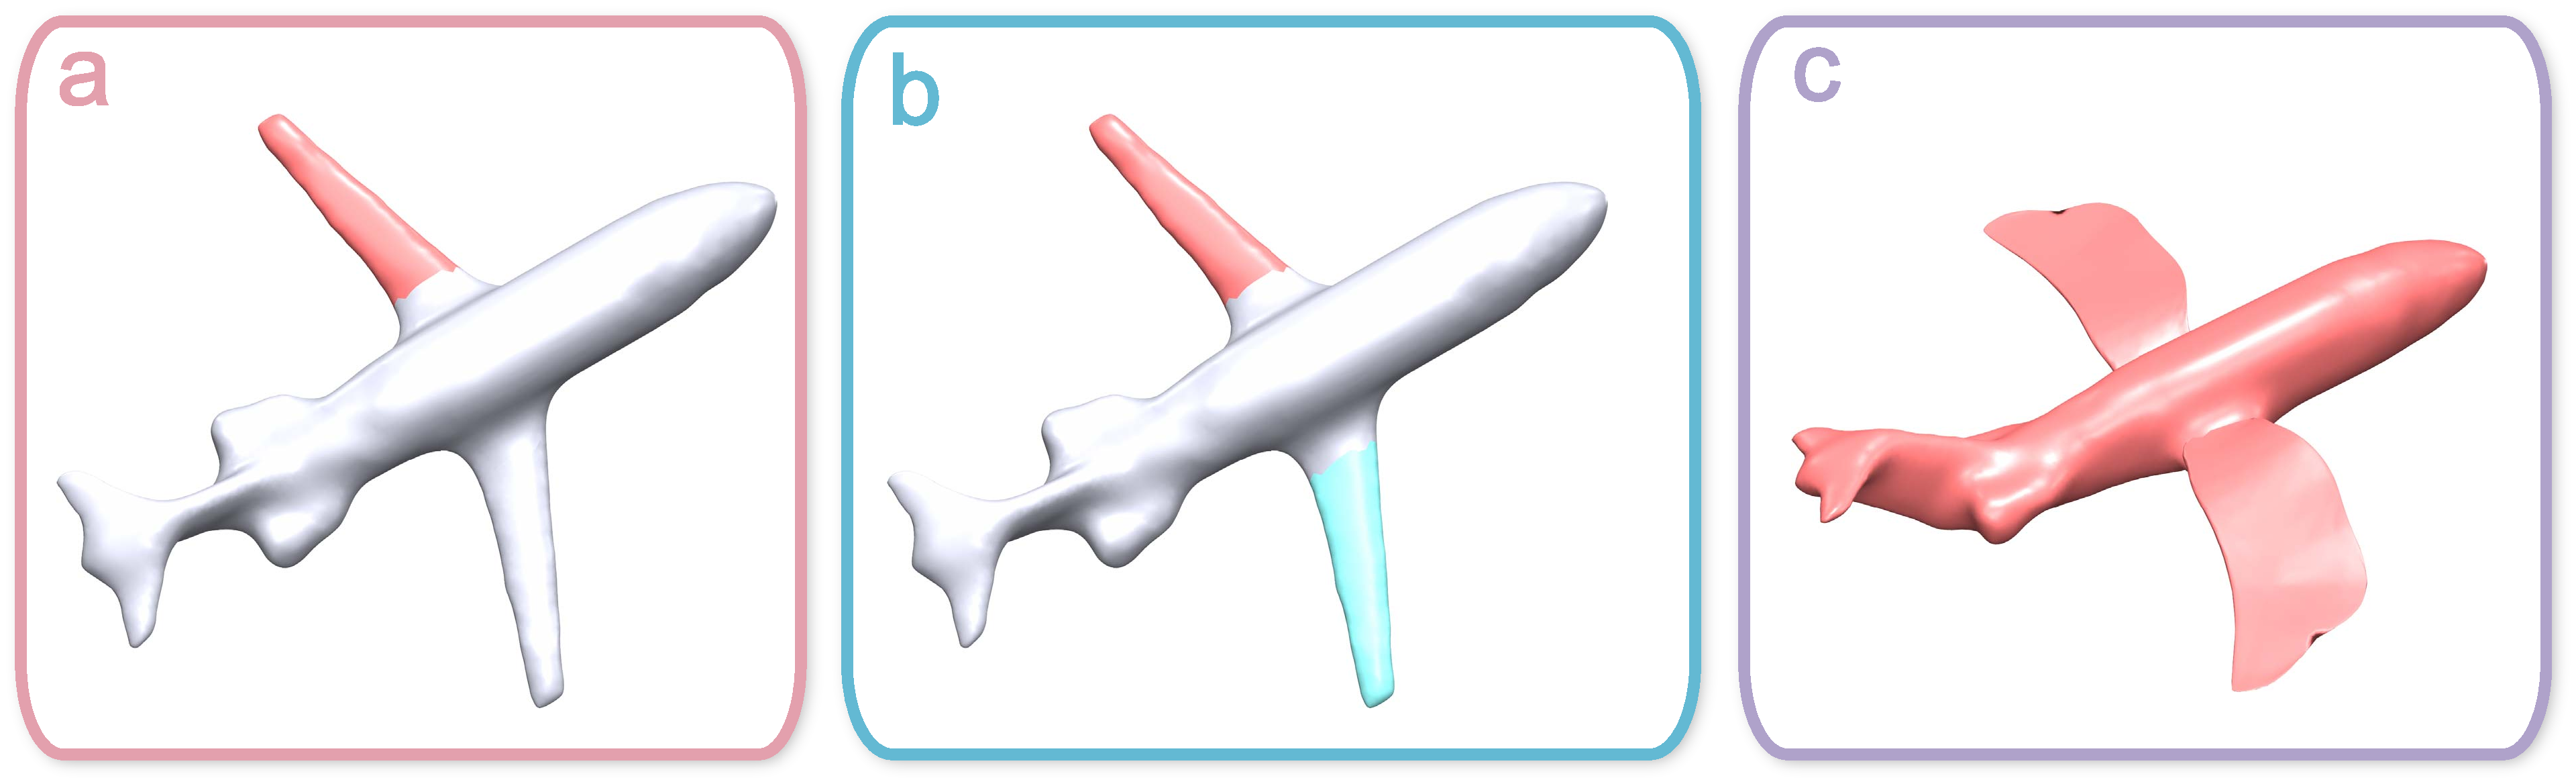
\includegraphics[width=1.0\linewidth]{./Material/SymSel.pdf}
\caption{Example of symmetry-aware selection and editing. The user selects an arbitrary region of a shape (a). Note that the region is not the complete wing, i.e. it is not a ``standard'' segment. We use our algorithm as a fast partial matching technique, to find other parts in the same shape with the same contour. This yields the corresponding region of the other wing as a symmetric counterpart (b). Finally, the symmetric pair may be replaced by another, retrieved from a database using our ``shape variations'' approach (c).}\label{fig:SymSel}
\end{figure}

\paragraph*{Symmetry-aware selection and editing.} Our method can also be used to select a group of similar elements in a single shape for further editing. For example, in Fig \ref{fig:SymSel}, the user picks an arbitrary region of the leg of a table. The corresponding regions of the other legs will be automatically identified, by partial matching of the contour of the selected region with the rest of the shape itself. Subsequently, the entire selected group can be replaced by similar parts retrieved from the database, as in the ``shape variations'' applicaton.

\paragraph*{Part suggestion.} Our on-the-fly part extraction technique can be used to suggest parts to extend a base shape~\cite{datadrivenvladenaisa2010,probabilisticreasoningvladlensg2011}. In contrast to previous methods, we do not require a pre-segmented database. Given a query shape, we treat its outline as the query contour and feed it to the algorithm. Our method matches the contour to parts of exemplar shapes, and suggests maximal connected components of the {\em rest} of the exemplar as suggestions for creatively extending the shape. The suggested parts can be irregular ones or from different shape families (see Figure \ref{fig:appl}).

\begin{figure}[t]\centering
\includegraphics[width=1.05\linewidth]{./Material/Appl.pdf}
\caption{Examples of part suggestions. Given the query shapes (in green), our system presents a list of part suggestions (in purple). The assembled shapes are shown below the suggested parts.}\label{fig:appl}
\end{figure}

\paragraph*{Multi-scale part suggestion.} Our system can suggest parts at various scales. Given a part \st{suggested} \hl{retrieved} by the method above, we perform normalized cuts~\cite{randomizedcutsfunkhousertog2008} on \hl{the SFG corresponding to the retrieved part} \st{its corresponding sub-SFG} to generate $T_n$ segments, each of which consists of a group of adjacent super-faces. $T_n$ is defined as:
\[{T_n} = \frac{{w(Vol(P_M)-Vol\left( {{p_p})} \right)}}{{Vol\left( {{p_p}} \right)}},\] where $Vol\left( \cdot \right)$ is the volume of an object, $P_M$ is the retrieved database model, $p_p$ is the part in the database model corresponding to the query \hl{(corresponding part)}, and the weight $w = 2$. We constrain $T_n$ to lie between 1 and 7. We rank the segments in ascending order by their distance to the corresponding part. \hl{The distance is defined as the Euclidean distance between the OBB of the segment and the corresponding part.} Now, given a scale $S$, we can suggest the segments \st{with this scale} \hl{, whose distance to the corresponding part is less than or equal to $S$}. An example is given in Figure \ref{fig:MSPS}.

\begin{figure}[t]\centering
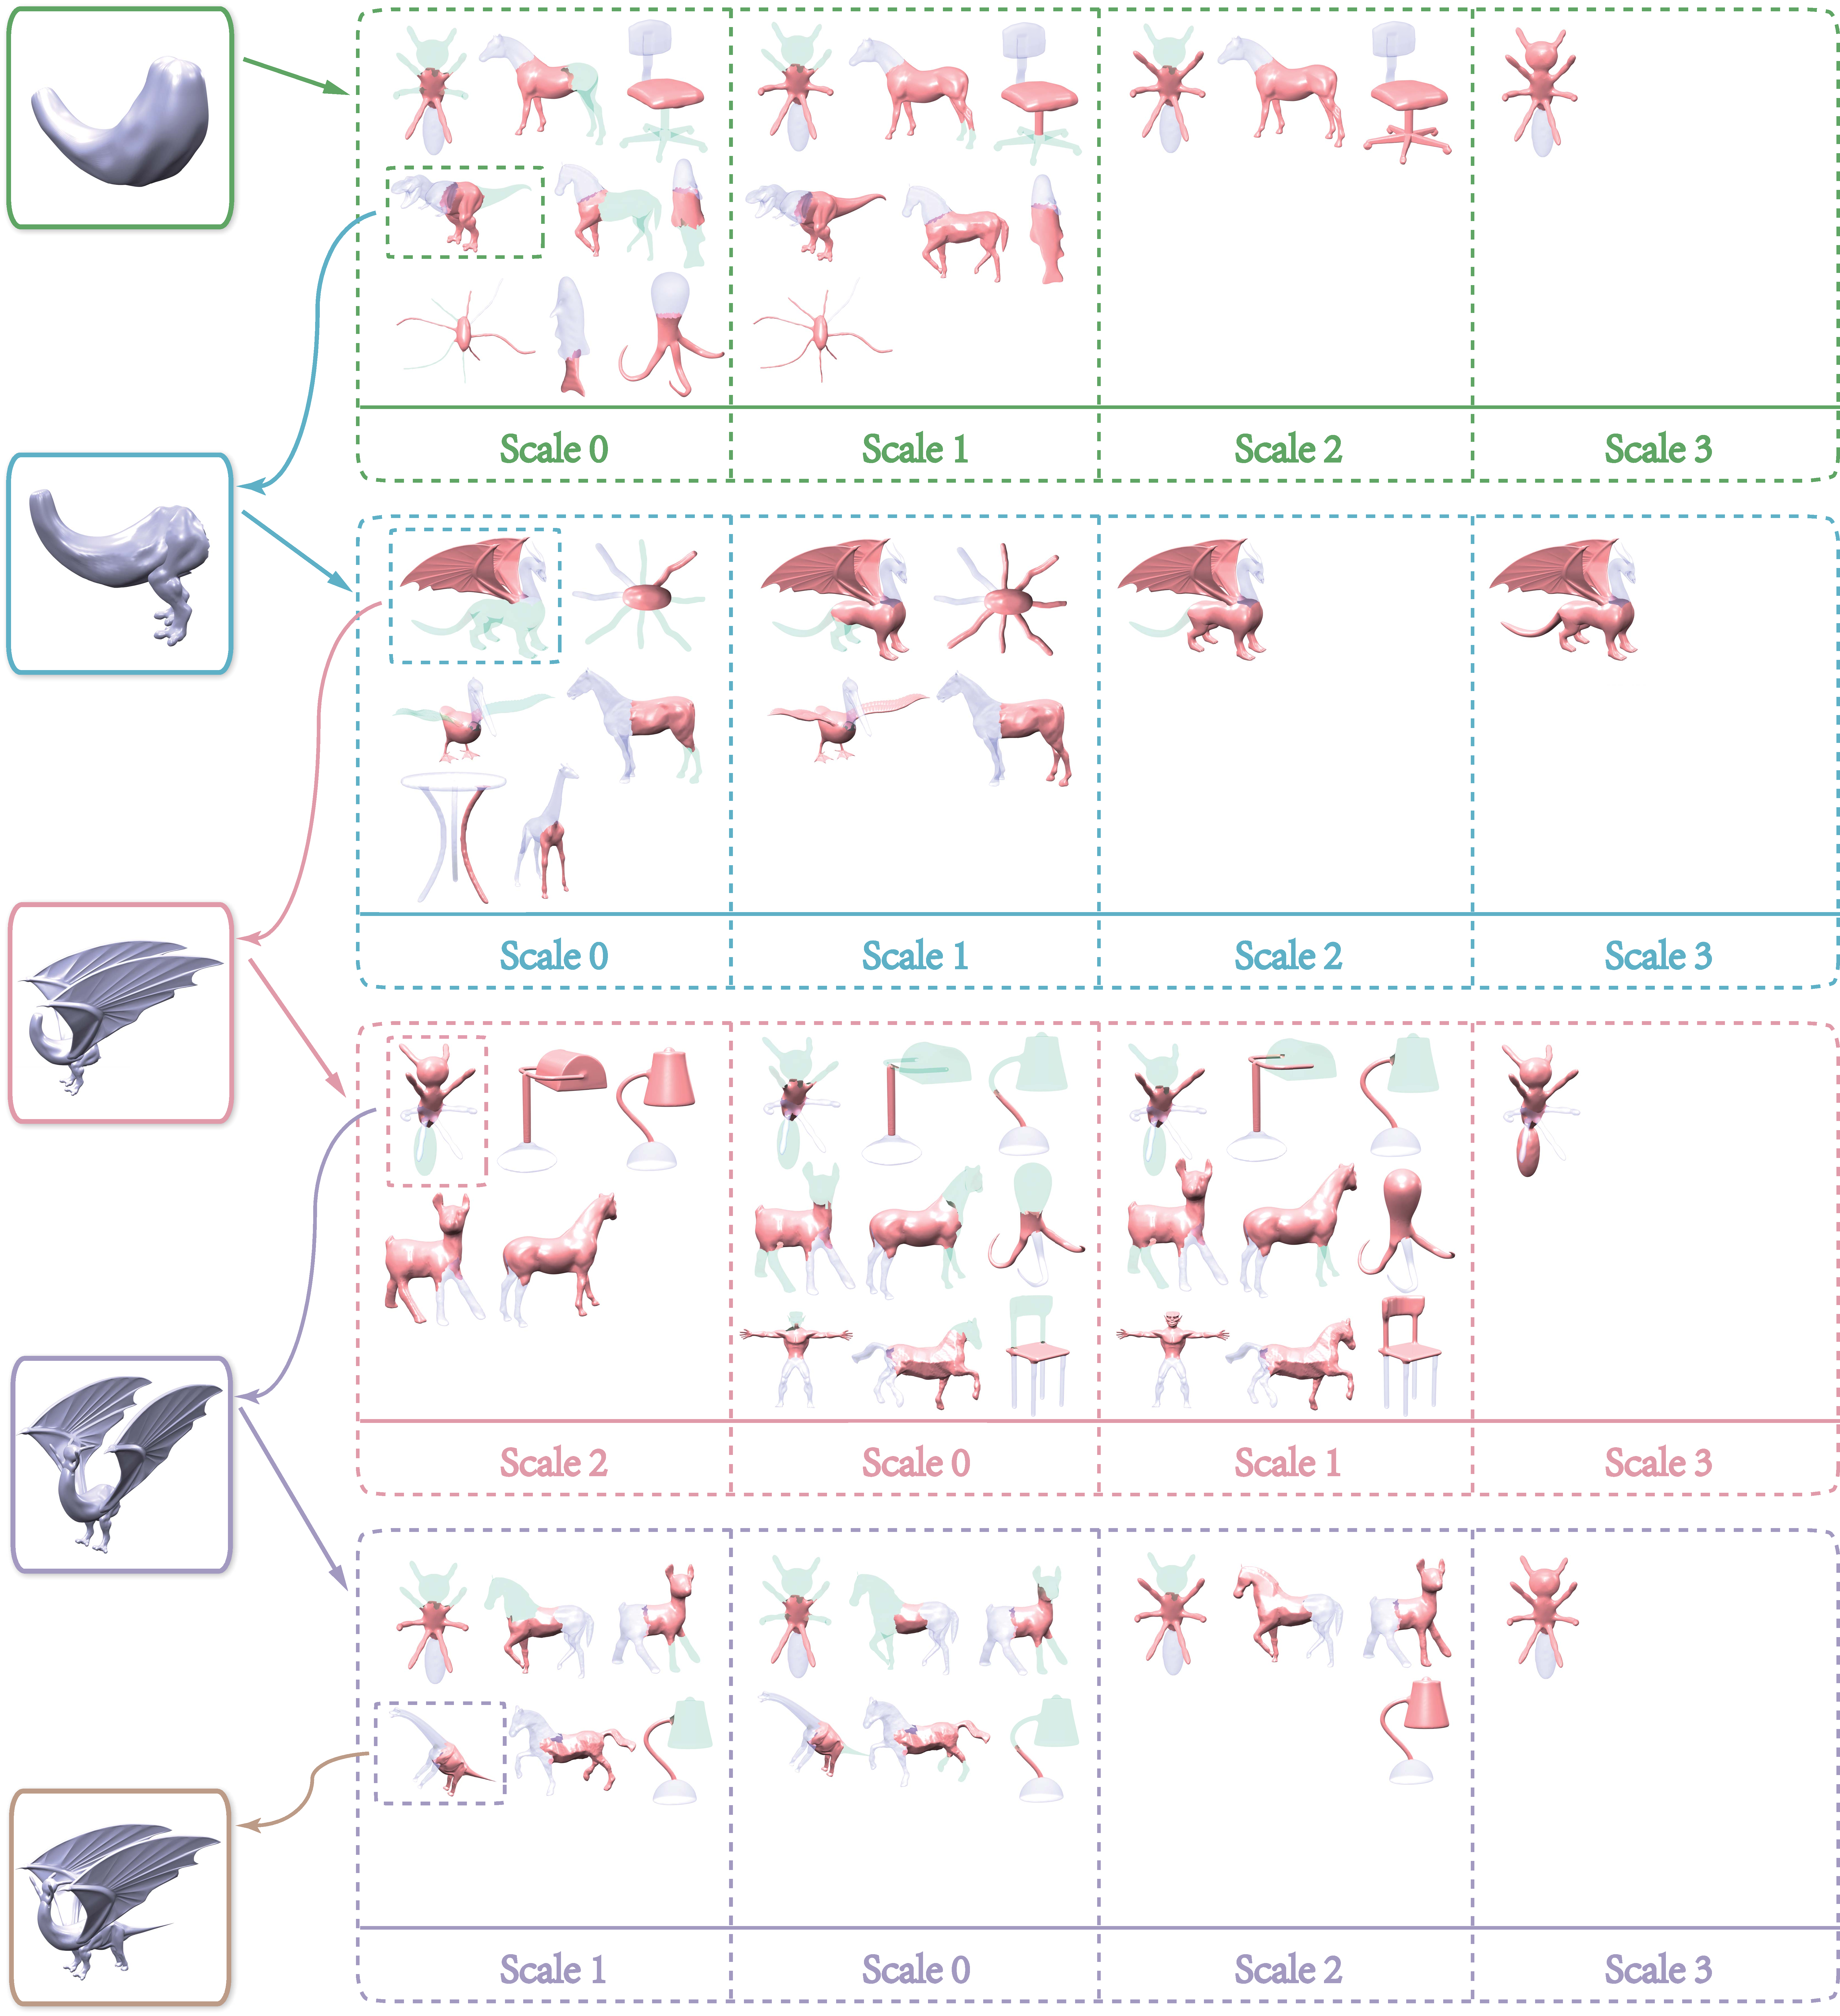
\includegraphics[width=1.05\linewidth]{./Material/MSPS.pdf}
\caption{An example of multi-scale part suggestion. The initial shape and subsequent working models, used as queries, are listed in the left column. On the right, we show the suggested parts (red) at different scales for each modeling step. The parts corresponding to the queries are marked in light blue. The other parts are marked in light green.}\label{fig:MSPS}
\end{figure}
